\documentclass[aspectratio=43]{beamer}

\usepackage[T1]{fontenc}
\usepackage[utf8]{inputenc}
\usepackage[english]{babel}
\usepackage{lmodern}
\usepackage{booktabs}
\usepackage{tcolorbox}
\usepackage{tikz}


%import the theme and packages for the code blocks
\input{code_blocks_theme.tex}

% Use Unipd as theme, with options:
% - pageofpages: define the separation symbol of the footer page of pages (e.g.: of, di, /, default: of)
% - logo: position another logo near the Unipd logo in the title page (e.g. department logo), passing the second logo path as option 
% Use the environment lastframe to add the endframe text
\usetheme[pageofpages=of]{Unipd}

\title{No U-Turn Sampler}
\subtitle{Adaptively Setting Path Lengths in Hamiltonian Monte Carlo}
\author[]{Pieripolli Leonardo, Pirazzo Tommaso, \\
			Ponchio Mattia, Secco Benedetto}

\date{\today}


\begin{document}

% Make the title page
\frame{\titlepage}

%--------------------------------------------------------------- project part
\section{Introduction}

\begin{frame}{No U-Turn Sampler}
	\begin{center}
		 
		\emph{HMC} is an \emph{MCMC} algorithm that avoids random walk behavior and sensitivity to correlated parameters.\\ %, by taking a series of steps informed by first-order gradient information. \\
		However, it requires the tuning of two user-specified parameters: step size $\epsilon$ and number of steps $L$. \\ 
		
		\pause
		%\vspace{1pt}
		\(\Downarrow\)
		\vspace{1pt}\\
		The \emph{No-U-Turn Sampler} (NUTS) is an extension to HMC that eliminates the need to set a number of steps $L$.
		
		\pause
		%\vspace{1pt}
		\(\Downarrow\)
		\vspace{1pt}\\
		\emph{NUTS} uses a recursive algorithm to build a set of candidate points, stopping automatically when it starts retrace its steps. 
		
		\pause
		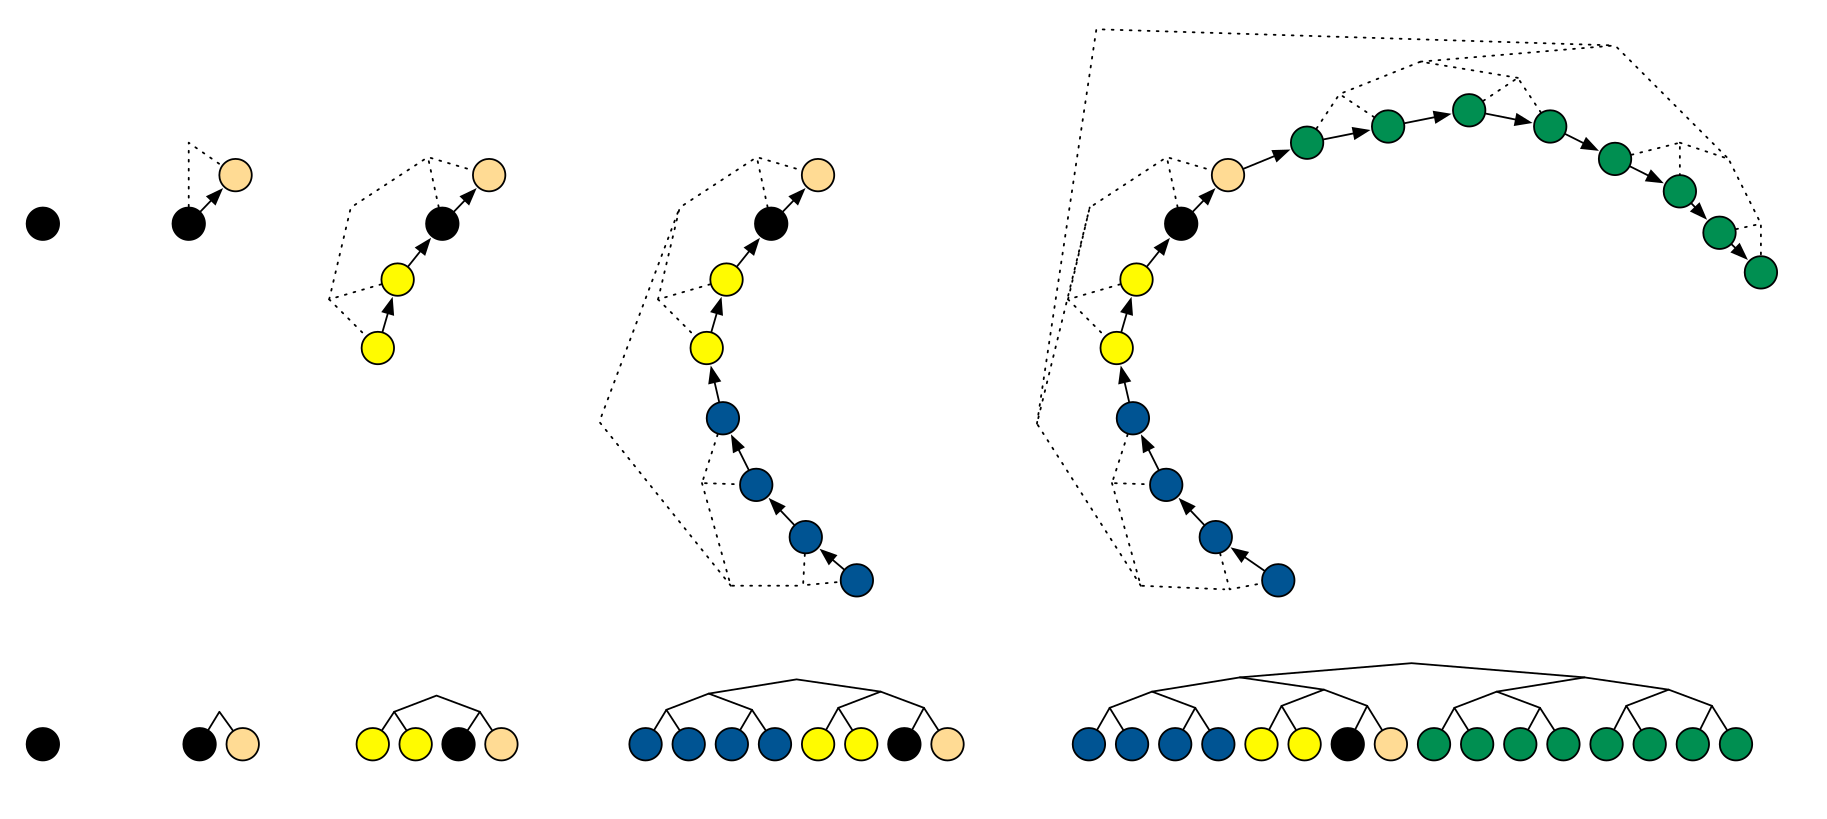
\includegraphics[width=0.6\textwidth]{images/immagini_leonardo/NUTS_diagram.png}
		
	\end{center}
	
\end{frame}

%----------------------------------------------------------------------------------------------------

\begin{frame}{Hamiltonian Monte Carlo}
	HMC generates proposals with high acceptance probability by suppressing the random walk behavior, but it comes with a price:
	\pause
	\begin{itemize}
		\item Comuputing the gradient of the log-posterior at each step. \\
		\pause
		\item Tuning two user-specified parameters: step size $\epsilon$ and number of steps $L$.
		Tipically, $\epsilon$ can be tuned during warm-up, but $L$ can require costly tuning runs. \\
	\end{itemize}
	\pause
	\centering
    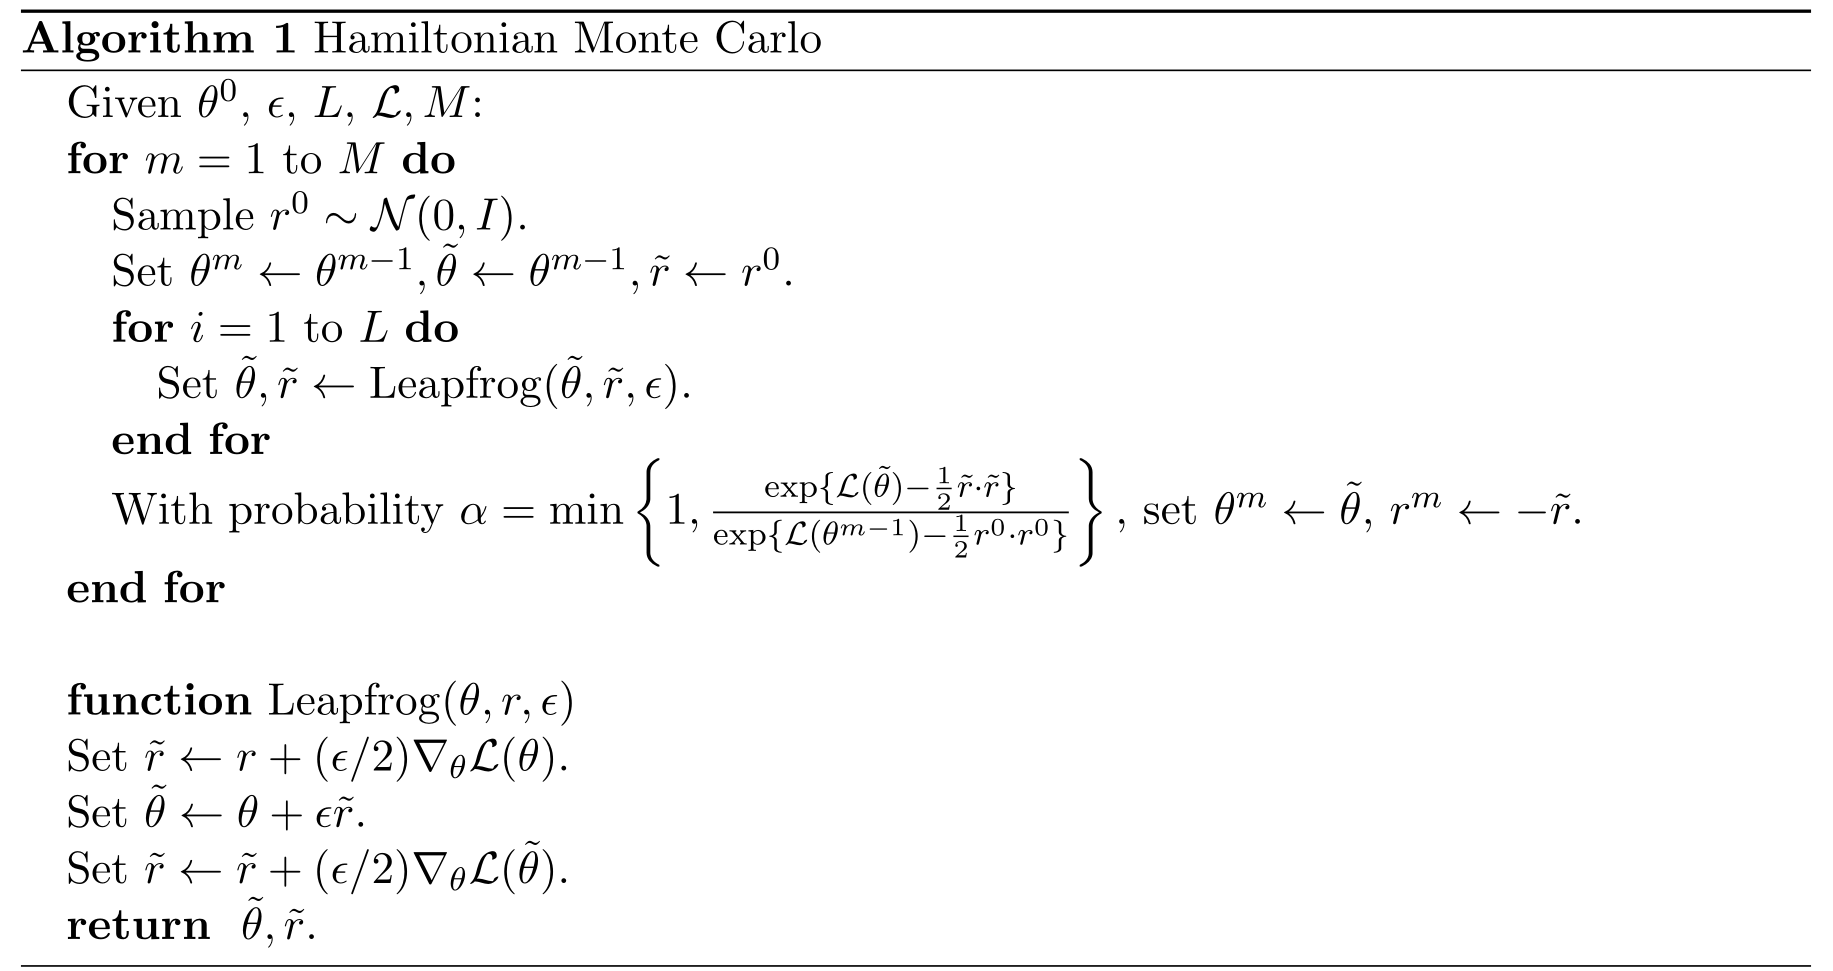
\includegraphics[width=0.75\textwidth]{images/immagini_leonardo/HMC.png}

\end{frame}

%----------------------------------------------------------------------------------------------------

\begin{frame}{No U-Turn HMC}
	We want a sampler able to retain the HMC suppression on random walk behavior, but without the need to tune the number of Leap Frog steps $L$. \\
	\pause
	\begin{itemize}
		\item Starting from a point in the parameter space $\theta$, the algorithm builds a set of candidate points, doubling the tree size at each iteration. \\
		\pause
		\item To detect when to stop, the algorithm checks if the trajectory starts to turn back on itself: given a proposed point $\tilde{\theta}$, the algorithm checks if the dot product of the momentum vectors at $\theta$ and $\tilde{\theta}$ is negative. \\
		$(\theta - \tilde{\theta}) \cdot \frac{d}{dt}(\theta - \tilde{\theta}) =(\theta - \tilde{\theta}) \cdot \tilde{r} < 0$ \\
		\pause
		\item To preserve time reversibility, NUTS runs the Hamiltonian dynamics in both forward and backward directions. \\
	\end{itemize}
	

\end{frame}

%----------------------------------------------------------------------------------------------------
\section{NUTS algorithm}

\begin{frame}{Probability slicing}
	\begin{center}
		 
		To simplify the derivation and implementation of the algorithm, NUTS uses a slice variable $u$ with conditional distribution $p(u|\theta, r) = \mathcal{U}(u; [0, exp{\mathcal{L}(\theta)-\frac{1}{2}r\cdot r}]) $. \\ 
		This way $p(\theta, r | u ) = \mathcal{U}(\theta, r; {\theta', r' | exp{\mathcal{L}(\theta)-\frac{1}{2}r\cdot r} \geq u})$. \\
		\pause
		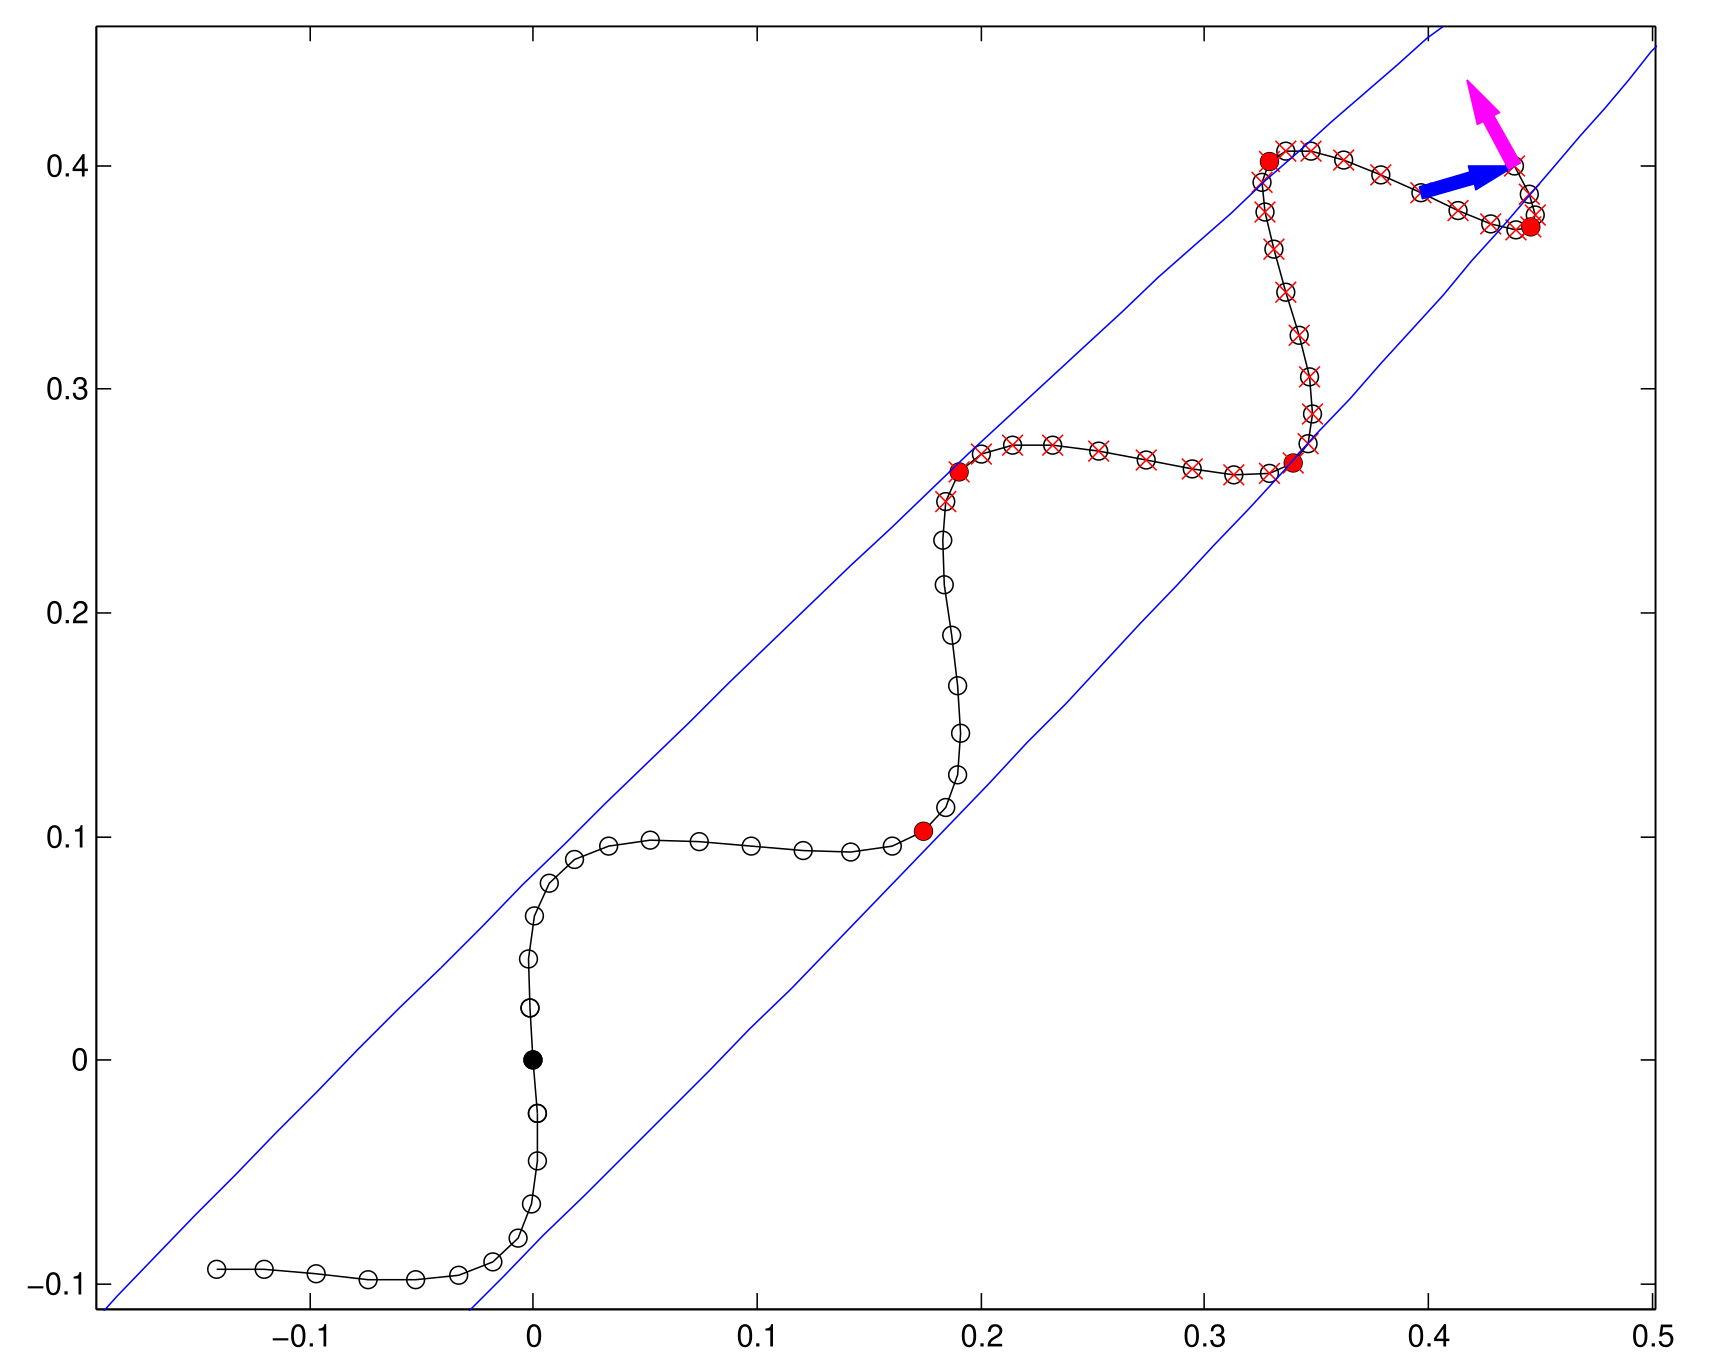
\includegraphics[width=0.65\textwidth]{images/immagini_leonardo/NUTS_example.png}
		
	\end{center}
	
\end{frame}

%----------------------------------------------------------------------------------------------------

\begin{frame}{High-levl NUTS algorithm}
	
	\begin{columns}

        \begin{column}{0.5\textwidth}
        \small
		
			\begin{itemize}
				\item The algorithm resamples $u|\theta, r$ at each iteration,
				\item uses Leapfrog integrator to trace a path forward and backwards first 1 step,
				\item then doubling for successive iterations.
				\item This doubling process implicitly builds a balanced binary tree whose leaf nodes correspond to position-momentum states.
				\item The doubling is halted when the subtrajectory starts to double back on itself.
				% \item At this point NUTS stops the simulation and samples from among the set of points.
			\end{itemize}

		\end{column}
		
        \begin{column}{0.5\textwidth}
            \centering
            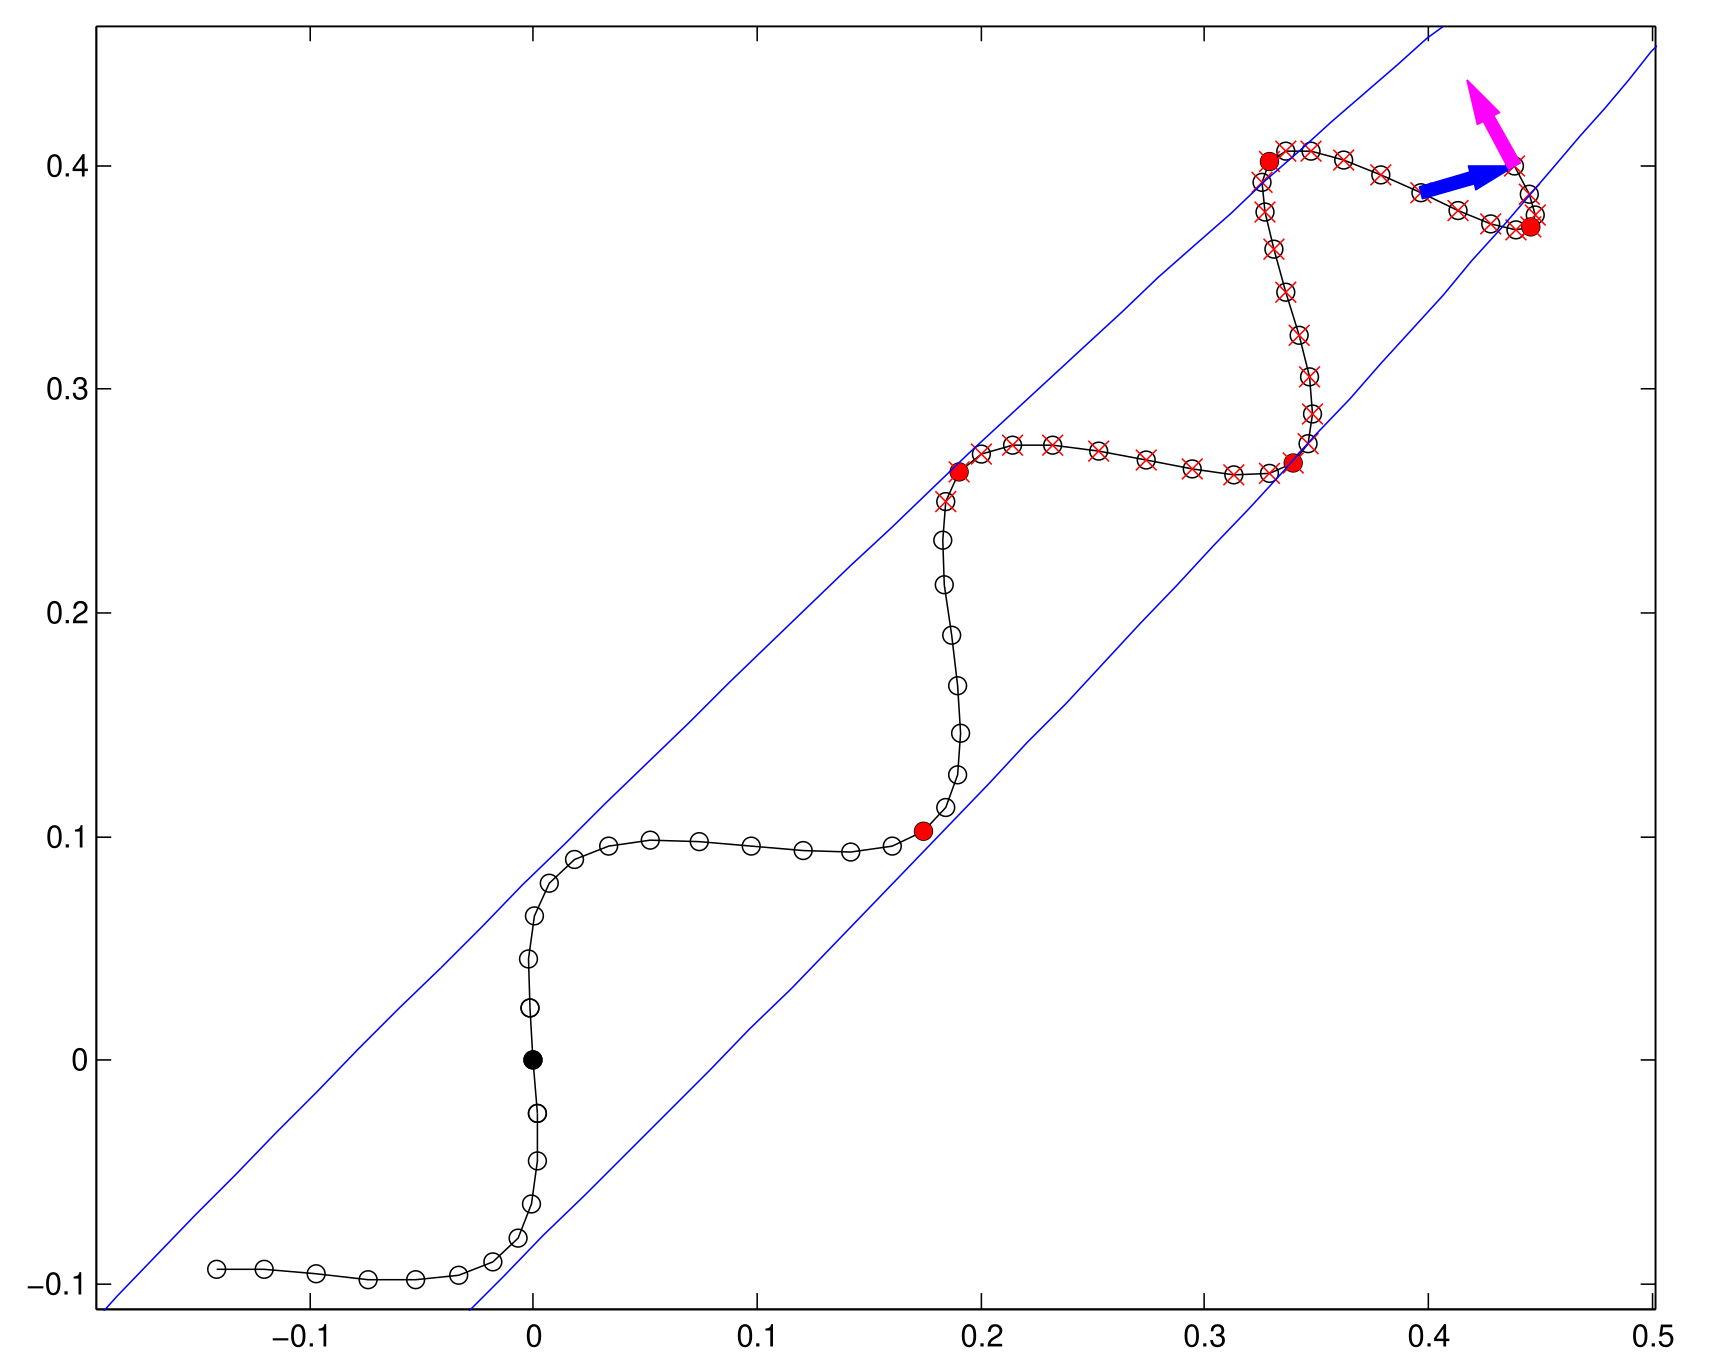
\includegraphics[width=1\textwidth]{images/immagini_leonardo/NUTS_example.png} \\
			\small 
			Example of a NUTS trajectory, with the slice variable $u$.
        \end{column}    
    \end{columns}

\end{frame}

%----------------------------------------------------------------------------------------------------


%  \begin{frame}{The cluster operative}
% 	\begin{tikzpicture}[remember picture,overlay]
% 		% Cloud Veneto - in alto a destra
% 		\node[anchor=north east] at ([xshift=-0.8cm,yshift=0.1cm]current page.north east) {
% 			
\includegraphics[width=2cm]{images/immagini_tommaso/cloud_veneto_logo.png}
% 		};
% 	\end{tikzpicture}

% 	\begin{columns}

%         \begin{column}{0.5\textwidth}
%         \small
		
% 			\begin{itemize}
% 				\item The cluster is started using \emph{Dask} function \texttt{SSHCluster}. 
% 				\item The scheduler connects to the workers using \emph{SSH} protocol, so that the workers can be started remotely.
% 				\item The scheduler is started on \textbf{ALICE} and it connects to the workers on the other machines, using their aliases, mapped to their IPs in the ssh configuration file.
% 			\end{itemize}

% 		\end{column}
% 		\pause
%         \begin{column}{0.5\textwidth}
%             \centering
%             \includegraphics[width=1.1\textwidth]{images/immagini_leonardo/Cluster_Details.png}
% 			\small 
% 			Specific properties of the running cluster
%         \end{column}    
%     \end{columns}
% \end{frame}

%----------------------------------------------------------------------------------------------------

% \begin{frame}{The "big data" problem}
	
% 	\begin{center}
		
% 		\begin{tcolorbox}[colback=blue!10, colframe=blue!60, rounded corners]
% 			\centering
% 			\Large{Inherent sequential nature of \emph{k-means++} !}	
% 		\end{tcolorbox}
		
% 		\pause
% 		\vspace{1pt}
% 		\(\Downarrow\)
% 		\vspace{1pt}\\
% 		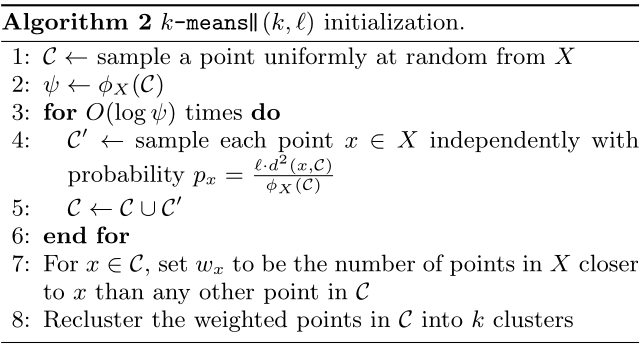
\includegraphics[width=1\textwidth]{images/immagini_tommaso/art_alg_02.png}
		
% 	\end{center}
		% \vspace{1pt}
		% \(\Downarrow\)
		% \vspace{1pt}\\
% \end{frame}


% % Model----------------------------------------------------------------------------------------------
% \begin{frame}{The datasets}
% 	We used two datasets to test and evaluate performances:
% 	\pause
% 	\begin{itemize}
% 		\item \textbf{Gaussian mixture}\\
% 			This dataset is made of $2 \times 10^6$ points (64 MB) in $N$ dimension and they are Gaussian distributed. To test the code we used also smaller versions of the dataset.
% 		\pause
% 		\item \textbf{KDD Cup 1999}\\
% 			This datset is commonly used in ML and in algorithms evaluation. It consist of $4.8 \times 10^6$ points (743 MB) in 42 dimensions. Three of them are categorical variables, so in the code we implemented a method to load the dataset without them or transform the categorial dimensions using the one-hot encoding standard. To test the code in local clusters we used a smaller version of the code importing only the $10\%$ of the dataset. 
% 	\end{itemize}
% \end{frame}


% \begin{frame}{Computational framework}
% 	\begin{tikzpicture}
		
% 		\pause
% 		% In alto a sinistra
% 		\node at ([xshift=-4cm,yshift=3cm]current page.center) {
% 			
\includegraphics[width=6cm]{images/immagini_tommaso/python_logo.png}
% 		};
		
% 		\pause
% 		% Python - in alto a destra
% 		\node at ([xshift=1cm,yshift=1.5cm]current page.center) {
% 			
\includegraphics[width=5cm]{images/immagini_tommaso/dask_logo.png}
% 		};
		
% 		\pause
% 		% Dask - in basso a sinistra
% 		\node at ([xshift=-4cm,yshift=-0.5cm]current page.center) {
% 			
\includegraphics[width=6cm]{images/immagini_tommaso/docker_logo.png}
% 		};
		
% 		\pause
% 		% Docker - in basso a destra
% 		\node at ([xshift=1.5cm,yshift=-2cm]current page.center) {
% 			
\includegraphics[width=4cm]{images/immagini_tommaso/cloud_veneto_logo.png}
% 		};
		
% 	\end{tikzpicture}
% \end{frame}


% % Model----------------------------------------------------------------------------------------------
% \begin{frame}{The Cluster Environment}
% 	To challenge the performances of the algorithm we decided to work on a small cluster on Cloud Veneto, runned on 4 Virtual Machines (VMs) with the following configuration:
% 	\begin{tikzpicture}[remember picture,overlay]
% 		% Cloud Veneto - in alto a destra
% 		\node[anchor=north east] at ([xshift=-0.8cm,yshift=0.1cm]current page.north east) {
% 			
\includegraphics[width=2cm]{images/immagini_tommaso/cloud_veneto_logo.png}
% 		};
% 	\end{tikzpicture}
% 	\pause
% 	\begin{itemize}
% 		\item \textbf{ALICE}: 2 CPU cores, 4 GB RAM, IP:220, alias \emph{scheduler}
% 		\begin{itemize}
% 			\item It hosts the \emph{scheduler} and \emph{client} of the cluster, it is the VM to which we connect from outside the cluster.
% 			\item It is used to host two \emph{Dask workers}, one for each CPU core.\\ 2 X (1 CPU core, 2 GB RAM)
% 		\end{itemize}
% 	\pause
% 		\item \textbf{WORKER1}: 1 CPU core, 2 GB RAM, IP:160, alias \emph{worker1}
% 		\item \textbf{WORKER2}: 1 CPU core, 2 GB RAM, IP:176, alias \emph{worker2}
% 		\item \textbf{WORKER3}: 1 CPU core, 2 GB RAM, IP:218, alias \emph{worker3}
% 	\end{itemize}
% 	\pause
	
% 	The total cluster can use a total of 5 CPU cores and 10 GB RAM, not very impressive compared to a modern laptop.
% \end{frame}

% %----------------------------------------------------------------------------------------------------


% \begin{frame}{The cluster setup}
% 	\begin{tikzpicture}[remember picture,overlay]
% 		% Cloud Veneto - in alto a destra
% 		\node[anchor=north east] at ([xshift=-0.8cm,yshift=0.1cm]current page.north east) {
% 			
\includegraphics[width=2cm]{images/immagini_tommaso/cloud_veneto_logo.png}
% 		};
% 	\end{tikzpicture}

% 	\begin{itemize}
% 		\item In each machine we ensured to have the same version of the \emph{OS} (ubuntu-24.04-noble-server), of \emph{Python} and related \emph{packages} (including the \emph{Dask} library and dependencies). \\
% 		\pause
% 		\item We used a \emph{Miniconda} environment with fixed versions of the packages, saved in a \emph{YAML} file.
% 	\end{itemize}

% 	\centering
%     \includegraphics[width=0.75\textwidth]{images/immagini_leonardo/Dask_dashboard_example.png}

% \end{frame}

% %----------------------------------------------------------------------------------------------------

% \begin{frame}{The cluster setup}
% 	\begin{tikzpicture}[remember picture,overlay]
% 		% Cloud Veneto - in alto a destra
% 		\node[anchor=north east] at ([xshift=-0.8cm,yshift=0.1cm]current page.north east) {
% 			
\includegraphics[width=2cm]{images/immagini_tommaso/cloud_veneto_logo.png}
% 		};
% 	\end{tikzpicture}
% 	To enable the parallelized read of the datasets, we established a network file system \emph{NFS}.
% 	\pause
% 	\begin{itemize}
% 		\item On \textbf{ALICE} was setup a nfs server, hosting a shared folder with the dataset, enabling the other machines to also write on it.
% 		\pause
% 		\item Each worker machine mounts the shared folder in the same path as the scheduler, so that the code can access the datasets without any modification.
% 		\pause
% 		\item The shared folder is mounted to be \textit{syncronous}, so that the read and write operations are done in a safe way, and with \textit{reconnectivity} attempts for robustness.
% 	\end{itemize}
% \end{frame}

% %----------------------------------------------------------------------------------------------------

% \begin{frame}{The cluster operative}
% 	\begin{tikzpicture}[remember picture,overlay]
% 		% Cloud Veneto - in alto a destra
% 		\node[anchor=north east] at ([xshift=-0.8cm,yshift=0.1cm]current page.north east) {
% 			
\includegraphics[width=2cm]{images/immagini_tommaso/cloud_veneto_logo.png}
% 		};
% 	\end{tikzpicture}

% 	\begin{columns}

%         \begin{column}{0.5\textwidth}
%         \small
		
% 			\begin{itemize}
% 				\item The cluster is started using \emph{Dask} function \texttt{SSHCluster}. 
% 				\item The scheduler connects to the workers using \emph{SSH} protocol, so that the workers can be started remotely.
% 				\item The scheduler is started on \textbf{ALICE} and it connects to the workers on the other machines, using their aliases, mapped to their IPs in the ssh configuration file.
% 			\end{itemize}

% 		\end{column}
% 		\pause
%         \begin{column}{0.5\textwidth}
%             \centering
%             \includegraphics[width=1.1\textwidth]{images/immagini_leonardo/Cluster_Details.png}
% 			\small 
% 			Specific properties of the running cluster
%         \end{column}    
%     \end{columns}
% \end{frame}

% %----------------------------------------------------------------------------------------------------

% \begin{frame}{The cluster mirror image}
% 	\begin{tikzpicture}[remember picture,overlay]
% 		% Cloud Veneto - in alto a destra
% 		\node[anchor=north east] at ([xshift=-0.8cm,yshift=-0.7cm]current page.north east) {
% 			
\includegraphics[width=3cm]{images/immagini_tommaso/docker_logo.png}
% 		};
% 	\end{tikzpicture}

% 	\begin{itemize}
% 		\item For the preliminary tests on developing functions, and to continue working while Cloud Veneto is not available, we created a mirror image of the cluster on our local machines using \emph{Docker} containers.
% 		\pause
% 		\item Staring from the same base image, made to match the cluster environment (OS, Python version, conda environment), we created a \textit{scheduler} image, a \textit{worker} image and a \textit{jupyter} (client) image, uploading them on \texttt{docker-hub}.
% 		\pause
% 		\item To mimic the cluster, we limited the resources of the containers to match the cluster ones, and we created a \texttt{Docker-compose} to allow the containers to communicate with each other via logical ports. \\
% 		(The dask cluster was not the same as the one on Cloud Veneto, but it was enough to test the code).
% 	\end{itemize}
	
% \end{frame}


\end{document}



